\subsection{Gyroskop}
Et gyroskop er et elektromekanisk apparat, som anvendes til at måle omdrejninger pr sekund eller vinkelhastighed om egen akse, hvilket kan ses på \figref{fig:gyro}. Enhederne for dette er henholdsvis revolutions per second (RPS) og $^\circ$/sek. Dette kan give information om orienteringen eller navigationen af objektet, som sensoren optager data fra. Hvis et gyroskop eksempelvis drejes én omgang om egen akse i sekundet, vil den registrere en vinkelhastighed på 360 grader pr sekund. \citep{Sparkfun_gyro}
\begin{figure}[H]
	\centering
	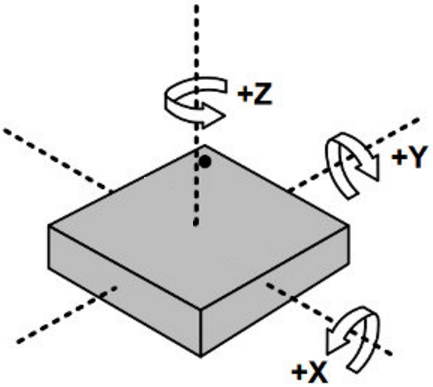
\includegraphics[scale=0.8]{figures/bProblemloesning/gyro.png}
	\caption{På figuren ses et gyroskops måling af rotation omkring egen akse. \citep{Sparkfun_gyro}(Modificeret)}
	\label{fig:gyro}
\end{figure}
Den præcise måde, hvorpå gyroskopet måler på, afhænger af dets type. Der findes blandt andet vibrations, elektrostatiske og kernemagnetisk resonans gyroskoper. \citep{LuingeVeltink2005,TittertonWeston2004} Et gyroskop kan for eksempel registrer vinkelhastighed ved at anvende tyngdekræften og en lille indre masse \citep{Sparkfun_gyro}. Hvis et gyroskop eksempelvis opsamler data, mens det er placeret proximalt for den laterale malleolus, vil massen blive udsat for en roterende bevægelse omkring en vandret akse. Massen vil blive henholdsvis tungere og lettere i processen på grund af ydre påvirkende kræfter, hvorfor outputtet vil komme til udtryk som en sinus hvis plottet i forhold til tiden. Outputtet er afhængig af tyngdekræftens påvirkning af massen, hvorfor et varierende output kræver en bevægelse. Uanset placering af gyroskopet vil det altså have et fast output.\\
%Et gyroskop fungere ved at anvende inerti egenskaberne der opstår når et hjul spindes med en høj hastighed. Ved at hjulet fastholder den samme retning omkring aksen, kan impulsmomentmomentet, dets inertiprodukt samt hastighed være med til at definere en referenceretning. 
%De fundementale principper bag virkningen af et gyroskop er blandt andet det gyroskopiske inerti, som er når hjulet drejer om sin egen akse og står vinkelret på aksen. impulsmomentet som er fordelingen af en masse på et rotor, hvor vinkelhastigheden også har en betydning, og præcession som er rotationen omkring egen akse. 
%De signaler som opfanges af et accelerometrer, inkluderer ikke signaler fra den roterende akse og derfor kan en præcis orientering ikke opfanges. For at forbedre nøjagtigheden, kan man anvende gyroskoper som et supplement til accelerometre .
%Et gyroskop måler vinkelhastighed, hvor ændringen i orientering kan måles ved at integrere vinkelhastigheden på baggrund af en algoritme. \citep{LuingeVeltink2005}